\documentclass{standalone}

\usepackage{tikz}
\usetikzlibrary{arrows.meta}

\begin{document}

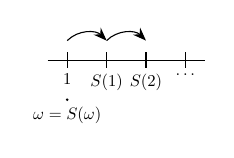
\begin{tikzpicture}[scale=0.5,>=Stealth]
  \draw (0.5,0) -- (4.5,0);

  \foreach \x/\label in {1/1, 2/S(1), 3/S(2), 4/\dots}
    \draw (\x,0.2) -- (\x,-0.2) node[below, scale=0.6] {$\label$};

  % Bended arrow from 1 to 2 (above)
  \draw[->, bend left=45] (1,0.5) to (2,0.5);

  % Bended arrow from 2 to 3 (above)
  \draw[->, bend left=45] (2,0.5) to (3,0.5);

  % omega
  \node[circle, fill=black, inner sep=0.2pt, label={[below, scale=0.6]below:$\omega = S(\omega)$}] (omega) at (1, -1) {};
    
\end{tikzpicture}

\end{document}